\documentclass{article}
\def\papertitle{Measurement Clusterization in Bayesian D-optimal Designs in Infinite Dimensions}
\def\authors{Yair Daon}
\def\journal{Bayesian Analysis}
\def\doi{12345}


% Define title defaults if not defined by user
\providecommand{\lettertitle}{Author Response to Reviews of}
\providecommand{\papertitle}{Title}
\providecommand{\authors}{Authors}
\providecommand{\journal}{Journal}
\providecommand{\doi}{--}

\usepackage[includeheadfoot,top=20mm, bottom=20mm, footskip=2.5cm]{geometry}

% Typography
\usepackage[T1]{fontenc}
\usepackage{times}
%\usepackage{mathptmx} % math also in times font
\usepackage{amssymb,amsmath}
\usepackage{microtype}
\usepackage[utf8]{inputenc}

% Misc
\usepackage{graphicx}
%% \usepackage[hidelinks]{hyperref} %textopdfstring from pandoc
\usepackage{soul} % Highlight using \hl{}

% Table

\usepackage{adjustbox} % center large tables across textwidth by surrounding tabular with \begin{adjustbox}{center}
\renewcommand{\arraystretch}{1.5} % enlarge spacing between rows
\usepackage{caption} 
\captionsetup[table]{skip=10pt} % enlarge spacing between caption and table

% Section styles

\usepackage{titlesec}
\titleformat{\section}{\normalfont\large}{\makebox[0pt][r]{\bf \thesection.\hspace{4mm}}}{0em}{\bfseries}
\titleformat{\subsection}{\normalfont}{\makebox[0pt][r]{\bf \thesubsection.\hspace{4mm}}}{0em}{\bfseries}
\titlespacing{\subsection}{0em}{1em}{-0.3em} % left before after

% Paragraph styles

\setlength{\parskip}{0.6\baselineskip}%
\setlength{\parindent}{0pt}%

% Quotation styles

\usepackage{framed}
\let\oldquote=\quote
\let\endoldquote=\endquote
\renewenvironment{quote}{\begin{fquote}\advance\leftmargini -2.4em\begin{oldquote}}{\end{oldquote}\end{fquote}}

\usepackage{xcolor}
\newenvironment{fquote}
  {\def\FrameCommand{
	\fboxsep=0.6em % box to text padding
	\fcolorbox{black}{white}}%
	% the "2" can be changed to make the box smaller
    \MakeFramed {\advance\hsize-2\width \FrameRestore}
    \begin{minipage}{\linewidth}
  }
  {\end{minipage}\endMakeFramed}

% Table styles

\let\oldtabular=\tabular
\let\endoldtabular=\endtabular
\renewenvironment{tabular}[1]{\begin{adjustbox}{center}\begin{oldtabular}{#1}}{\end{oldtabular}\end{adjustbox}}


% Shortcuts

%% Let textbf be both, bold and italic
%\DeclareTextFontCommand{\textbf}{\bfseries\em}

%% Add RC and AR to the left of a paragraph
%\def\RC{\makebox[0pt][r]{\bf RC:\hspace{4mm}}}
%\def\AR{\makebox[0pt][r]{AR:\hspace{4mm}}}

%% Define that \RC and \AR should start and format the whole paragraph 
\usepackage{suffix}
\long\def\RC#1\par{\makebox[0pt][r]{\bf RC:\hspace{4mm}}\textbf{\textit{#1}}\par} %\RC
\WithSuffix\long\def\RC*#1\par{\textbf{\textit{#1}}\par} %\RC*
\long\def\AR#1\par{\makebox[0pt][r]{AR:\hspace{10pt}}\textit{#1}\par} %\AR
\WithSuffix\long\def\AR*#1\par{\textit{#1}\par} %\AR*


%%%
%DIF PREAMBLE EXTENSION ADDED BY LATEXDIFF
%DIF UNDERLINE PREAMBLE %DIF PREAMBLE
\RequirePackage[normalem]{ulem} %DIF PREAMBLE
\RequirePackage{color}\definecolor{RED}{rgb}{1,0,0}\definecolor{BLUE}{rgb}{0,0,1} %DIF PREAMBLE
\providecommand{\DIFadd}[1]{{\protect\color{blue}\uwave{#1}}} %DIF PREAMBLE
\providecommand{\DIFdel}[1]{{\protect\color{red}\sout{#1}}}                      %DIF PREAMBLE
%DIF SAFE PREAMBLE %DIF PREAMBLE
\providecommand{\DIFaddbegin}{} %DIF PREAMBLE
\providecommand{\DIFaddend}{} %DIF PREAMBLE
\providecommand{\DIFdelbegin}{} %DIF PREAMBLE
\providecommand{\DIFdelend}{} %DIF PREAMBLE
%DIF FLOATSAFE PREAMBLE %DIF PREAMBLE
\providecommand{\DIFaddFL}[1]{\DIFadd{#1}} %DIF PREAMBLE
\providecommand{\DIFdelFL}[1]{\DIFdel{#1}} %DIF PREAMBLE
\providecommand{\DIFaddbeginFL}{} %DIF PREAMBLE
\providecommand{\DIFaddendFL}{} %DIF PREAMBLE
\providecommand{\DIFdelbeginFL}{} %DIF PREAMBLE
\providecommand{\DIFdelendFL}{} %DIF PREAMBLE
%DIF END PREAMBLE EXTENSION ADDED BY LATEXDIFF

\usepackage{amssymb,amsmath,amsthm,amsaddr}
\usepackage{thmtools}
\usepackage{thm-restate}

\usepackage{tikz,pgfplots,pgfplotstable}
\pgfplotsset{compat=1.9} % set to 1.8 to get old behaviour

%% %% % Graphics:
%% \usepackage[final]{graphicx}
\usepackage{graphicx} % use this line instead of the above to suppress graphics in draft copies
\usepackage{wrapfig}
%\usepackage{graphpap} % \defines the \graphpaper command
\usepackage[T1]{fontenc} % Use 8-bit encoding that has 256 glyphs
\usepackage[english]{babel} % English language/hyphenation


\usepackage{cite}
% makes color citations
\usepackage[colorlinks=true,urlcolor=blue,citecolor=red,linkcolor=red,bookmarks=true]{hyperref}
\usepackage{url}
\usepackage{color}
\usepackage{paralist}
%% \usepackage{graphics} %% add this and next lines if pictures should be in esp format
%% \usepackage{epsfig} %For pictures: screened artwork should be set up with an 85 or 100 line screen
\usepackage{epstopdf} 

%% From slides file
\usepackage{booktabs} % Allows the use of \toprule, \midrule and \bottomrule in tables
\usepackage[normalem]{ulem}
\usepackage{xcolor}
%\usepackage{algorithm}
%\usepackage[noend]{algpseudocode}
\usepackage{proof-at-the-end}

% Indent first line of each section:
\usepackage{indentfirst}

%% %% % Fonts and symbols:
\usepackage{amsfonts}


%% % Formatting tools:
%% %\usepackage{relsize} % relative font size selection, provides commands \textsmalle, \textlarger
%% %\usepackage{xspace} % gentle spacing in macros, such as \newcommand{\acims}{\textsc{acim}s\xspace}

%% % Page formatting utility:
%% \usepackage{geometry}
%% %\usepackage[margin=0.1in]{geometry}


%% Place here your \newcommand's and \renewcommand's. Some examples already included.
%\renewcommand{\le}{\leqslant}
%\renewcommand{\ge}{\geqslant}
%\renewcommand{\emptyset}{\ensuremath{\varnothing}}
%\newcommand{\ds}{\displaystyle}
\newcommand{\R}{\ensuremath{\mathbb{R}}}
%\newcommand{\Q}{\ensuremath{\mathbb{Q}}}
%\newcommand{\Z}{\ensuremath{\mathbb{Z}}}
%\newcommand{\N}{\ensuremath{\mathbb{N}}}
%\newcommand{\T}{\ensuremath{\mathbb{T}}}
%\newcommand{\B}{\mathcal{B}}
\newcommand{\eps}{\varepsilon}
%\newcommand{\closure}[1]{\ensuremath{\overline{#1}}}
\newcommand{\M}{\mathcal{M}}

\newcommand{\ep}{\varepsilon}
%\newcommand{\eps}[1]{{#1}_{\varepsilon}}
\newcommand{\bs}{\boldsymbol}
\newcommand{\der}{\text{\textup{d}}}
\newcommand{\coder}[1]{\texttt{#1}}
\newcommand{\inner}[2]{#1 \cdot #2}
\newcommand{\var}{\textup{Var}}
\newcommand{\corr}{\textup{Corr}}
\newcommand{\cov}{\textup{Cov}}
\newcommand{\diag}{\textup{diag}}
%% \newcommand{\dom}{\mathcal{D}om}
%% \newcommand{\note}[1]{{\textcolor{blue}{#1}}}
%% \newcommand{\A}[1]{{\textcolor{cyan}{\noindent Answer: #1}}}
%\newcommand{\reftwo}[1]{{\textcolor{green}{#1}}}
%\newcommand{\refthree}[1]{{\textcolor{red}{#1}}}
%% \newcommand{\refthree}[1]{{\color{red} #1}}
%% \newcommand{\reftwo}[1]{{\color{green} #1}}



%% \newcommand{\precop}{\mathcal{L}}
%% \newcommand{\precmat}{\mathbf{L}}
%% \newcommand{\Op}{\mathcal{A}}
%% \newcommand{\OpDir}{\mathcal{A}_{\textup{Dirichlet}}}
%% \newcommand{\OpNeu}{\mathcal{A}_{\textup{Neumann}}}
%% \newcommand{\covop}{\mathcal{C}}
%% \newcommand{\lag}{\mathcal{L}}
%% \newcommand{\n}{\boldsymbol{n} }
%% \newcommand{\dn}{\partial \n }
\newcommand{\x}{\mathbf{x}}
\newcommand{\y}{\mathbf{y}}
%% \newcommand{\z}{{\boldsymbol{z}}}
%% \newcommand{\kxmy}{ \kappa \| \x - \y \| }
%% \newcommand{\xmy}{ \| \x - \y \| }
%% \newcommand{\proj}{\mathcal{P}}
%% \newcommand{\kr}{\kappa r}
%% \newcommand{\ivar}{\text{IntVar}}

%% \newcommand{\K}{\mathbb{K}}
\newcommand{\hil}{\mathcal{H}}
%% \newcommand{\ban}{\mathcal{B}}
\newcommand{\hilp}{\mathcal{H}_p}
\newcommand{\hilo}{\mathcal{H}_o}
\newcommand{\obs}{\mathcal{O}}
\newcommand{\pobs}{\mathcal{P}}
\newcommand{\fwd}{\mathcal{F}}
%% \newcommand{\tru}{\fwd_{\textup{True}}}
%% \newcommand{\err}{\fwd_{\textup{Error}}}

\newcommand{\obsm}{\widehat{\obs}}
\newcommand{\Sigmam}{\widehat{\Sigma}}
\newcommand{\postcovm}{\widehat{\Gamma_{\textup{post}}}}
\newcommand{\uu}{\mathbf{u}}
\newcommand{\tar}{\Psi}
\DeclareMathOperator*{\argmin}{arg\,min}
\DeclareMathOperator*{\argmax}{arg\,max}

% Definitions for second chapter
\newcommand{\data}{\mathbf{d}}
\newcommand{\param}{\mathbf{m}}
\newcommand{\sspar}{\param_{\textup{SmallScale}}}
\newcommand{\normal}{\mathcal{N}}
\newcommand{\pr}{\mu_{\textup{pr}}} %Prior measure
\newcommand{\post}{\mu_{\textup{post}}^{\data, \obs}} % Posterior measure
\newcommand{\prmean}{\param_{\textup{pr}}} % Prior mean
\newcommand{\postmean}{\param_{\textup{post}}} % Posterior mean
\newcommand{\postcov}{\Gamma_{\textup{post}}} % Posterior covariance
\newcommand{\prcov}{\Gamma_{\textup{pr}}} % Prior covariance
\newcommand{\modcov}{\Gamma_{\textup{model}}} % Model covariance
\newcommand{\tmp}{\mathcal{G}}
\newcommand{\meas}{\mathbf{o}}
\newcommand{\ev}{\mathbf{e}} % eigenvector 
\newcommand{\func}{\mathbf{a}}
\newcommand{\tr}[1]{\textup{tr}\left \{#1 \right \} }
\newcommand{\ttr}[1]{\textup{tr}\ #1}
\newcommand{\rank}{\textup{rank}\ }
\newcommand{\des}{\eta} % vector of design parameters
\newcommand{\sigsqr}{\sigma^2}
%\newcommand{\acim}{\textsc{acim}\xspace}
%\newcommand{\acims}{\textsc{acim}s\xspace}


%% %% \newcommand\numberthis{\addtocounter{equation}{1}\tag{\theequation}}
%% %% %%
%% %% %% Place here your \newtheorem's:
%% %% %%
\newtheorem{theorem}{Theorem}
\newtheorem{definition}{Definition}

%% %% %% Some examples commented out below. Create your own or use these...
%% %% %%%%%%%%%\swapnumbers % this makes the numbers appear before the statement name.
%% %% %\theoremstyle{plain}
%% %% %\newtheorem{thm}{Theorem}[chapter]
\newtheorem{proposition}{Proposition}
\newtheorem{lemma}{Lemma}
\newtheorem{corollary}{Corollary}
%% %% % \newtheorem{observation}[theorem]{Observation}

%% %% %\theoremstyle{definition}
%% %% %\newtheorem{define}{Definition}[chapter]

%% %% %\theoremstyle{remark}
%% %% %\newtheorem*{rmk*}{Remark}
%% %% %\newtheorem*{rmks*}{Remarks}

%% %% %% Hack
%% %% \newcommand{\stkout}[1]{\ifmmode\text{\sout{\ensuremath{#1}}}\else\sout{#1}\fi}
%% %% \usepackage{cancel}

\usepackage{comment}% http://ctan.org/pkg/comment
%% %% %\excludecomment{proof}
%% \excludecomment{figure}
%% \let\endfigure\relax


\overfullrule=0pt

\usepackage{xr}
\externaldocument{ba}

\begin{document}

% Make title
{\Large\bf \lettertitle}\\[1em]
{\huge \papertitle}\\[1em]
{\authors}\\
{\it \journal, }\texttt{doi:\doi}\\
\hrule

% Legend
\hfill {\bfseries RC:} \textbf{\textit{Reviewer Comment}},\(\quad\) AR: \emph{Author Response}, \(\quad\square\) Manuscript text

I appreciate the many thoughtful comments by all of you. I believe
these comments helped me considerably improve the exposition of my
paper and added new insights as well. I sincerely appreciate the
option to revise and resubmit. Please see below my answers to the
comments made by the referees, associate editor and editor in chief:
\rred{My answers are marked in red.} \bblue{In some places I copied
  text from the revised manuscipt and marked it in blue.}



\section{Editor in Chief}
\RC Personally I like the paper, but it represents a somehow unusual
submission for Bayesian Analysis, and I am worried about it being of
sufficient general interest for the broad readership of the
journal. Still, in agreement with the AE, we decided to give the
author the possibility to revise the paper. However, I must stress
that there is no guarantee of a successful outcome, which will solely
depend on the quality of the revision. In particular:

\RC the Introduction is to be made accessible to the whole BA
    readership;
    
\AR  I have considerably extended the introduction.
   
    
\RV the motivation and the practical statistical implications are to
be developed and discussed;

\AR I added a section on the implications:
\begin{quote}
  Our answer to Question \ref{q:generic} implies that encountering
clusterization should be expected in many different problems across
many different scientific fields. Researchers that encounter
clusterization should not be surprised or wary. In Our answer to
Question \ref{q:why}, we explain what our view of the cause of
clusterization is. It appears, the cause is generic: a D-optimal
design reduces uncertainty for a select set of prior covariance
eigenvectors --- those with the most prior uncertainty, i.e.~those the
practitioner cares about the most! We believe practitioners should not
try to avoid measurement clusterization. Rather, practitioners should
take repeated measurements (e.g.~in MRI and borehole tomography),
increase apparatus sensitivity (e.g.~in EIT), or take consecutive
measurements (e.g.~in the 1D heat equation). Overall, we show that
measurement clusterization is a natural and (almost) inevitable part
of Bayesian D-optimal designs (but see disclaimer below).

One interesting implication of the analysis presented here is that
clusterization can serve as an evidence to the number of relevant
eigenvectors. Since leading eigenvectors typically correspond to slow
variations in space and/or time, clusterization could be used to
estimate the number of relevant degrees of freedom, and even to reduce
the complexity of a computational model, e.g.~by dropping
discretization points.

It is important to note that we do not view clustered designs as
undesirable, nor do we believe D-optimal designs should be avoided at
all. Nothing in our analysis indicates that we should expect any
pathological behavior when utilizing D-optimal designs. On the
contrary: we show that D-optimal designs (clustered or not) reduce
uncertainty of prior covariance eigenvectors where it is
highest. Thus, in a sense we hope to make precise in a future study,
we expect convergence of for D-optimal designs to be fastest.

For example, \cite{tekentrup2020} provides convergence analysis for
various designs with differing space filling properties. She showed
that convergence rate depends on how these designs fill space. We
expect better convergence rates for D-optimal designs; Even though
D-optimal desgins demonstrate clusterization, they do so because they
explore space in a way tailored to the problem studied. Consequently,
D-optimal designs cluster because they first aim to measure what
matters most; see the discussion following Theorem \ref{thm:char} for
details.



We expect D-optimal designs to judicious exploration of
design space, as implemented by a D-optimal design to give better
convergence compared to randomly sampling the design
space \cite{knapik2011}.




Clusterization is a peculiar phenomenon and it is perfectly reasonable
for someone to argue against the D-optimality criterion based on the
fact that it results in clustered designs. We have seen, however that
there is a perfectly reasonable explanation for clusterization. We
have shown that clusterization is an inevitable consequence of having
a problem with some modes where uncertainty decays faster than others.

Lastly, we believe that when clusterization arises, it should serve as
a warning sign to practitioners. In the inverse problem of the 1D heat
equation, clusterization occurs primarily because Laplacian
eigenvectors \emph{do not} decay in $\Omega$. Consequently, measuring
$u(x_1, T)$ at some point $x_1 \in \Omega$ provides information about
$u(x_2,T)$ for distant points $x_2 \in \Omega$. Intuitively, this
should not occur: for small $T$, the heat distribution at $x_1$ should
give very little knowledge on the heat distribution at $x_2$. This
behavior stems from a well-known property of the heat equation: it
allows information to spread \emph{instantly} across the computational
domain \cite{renardy2006PDE}. In reality, heat (and information)
propagate at finite speeds. Of course, the known physical barrier for
information spread is the speed of light, but we expect heat to spread
considerably slower: heating an Olympic pool at one end should have no
immediate effect on the temperature at the other end.

Our choice of prior is also a potential major contributor to
clusterization. Our choice of Gaussian prior similarly implies
information is shared between distant locations in $\Omega$. Thus, we
suggest refraining from choosing Gaussian priors with inverse
Laplacian covariance operators. Rather, non-Gaussian priors could be
employed instead \cite{hosseini2017, hosseini2019}.

We believe that the emergence of clusterization in this context is
thus non-physical, arising from the way the inverse problems we
consider are phrased. Clusterization therefore indicates that the
underlying mathematical / Bayesian model is overly permissive and
fails to capture crucial physical constraints of the problem. We
suggest that when clusterization occurs, practitioners should consider
alternative models where information is localized in space and travels
at finite speed in the medium. Such models may not only provide more
physically accurate and meaningful results but may also mitigate the
issue of clusterization.

\end{quote}
   
    
\RC the contribution has to be better contextualized with respect to
the literature in both inverse problems and D-optimal designs;

    
\RC numerical evidence and code, mentioned in the paper but actually
not provided, need to be made available;
    
\AR I added a section describing numerical experiments and their
results. I also added documentation to the accompanying
\href{https://github.com/yairdaon/OED}{repository} and made sure all
scripts there run.
    
    
\RC the mathematical derivations have to be watertight and some
clarifications are needed in this respect (see Report of Referee 3).
    

\AR I am not sure which specific comment of Reviewer 3 this
      refers to, please see my answers to Reviewer 3 below.
   

\section{Associate Editor}
\RC The three referees found merits and interest in your work, but also
pointed out several major issues to be addressed. Of particular
concern to me, the paper's exposition jumps too quickly into the
formulation / maths without giving a proper intuition and
context. This makes the paper less accessible to readers who aren't
already quite familiar with inverse problems (which are introduced
with very little preamble, and it's not even immediately explicit what
are the parameters being learned) and optimal experimental design.

\AR I have added considerably to the introduction. See revised
manuscript and diff file.


\RC A referee makes valid points as to whether clusterization of
measurements is a problem in general, when in fact in can be an
appealing feature in some settings, and another referee asks whether
D-optimal designs should be abandoned altogether. The exposition
needs to discuss these high-level issues, and introduce the related
literature and results appropriately, to give the work proper
context.



\RC Altogether, I think that your work has the potential to make a
good contribution to Bayesian analysis, but as it currently stands
significant work is needed.



\section{Referee 1}\label{ref1}
\RC This paper explains a common practical issue: the cause of
clusterization in Bayesian D-optimal designs in infinite dimensions
and why adding a correlated measurement process decluster the design
points. Its theoretical results are valuable to the field of inverse
problems/uncertainty quantification and the conclusions should be
useful to practitioners in this field.

\AR I appreciate the kind words.


\RC However, I feel changing the assumption from independent to correlated
measurements is quite artificial: people tweak a data generation
process assumption to solve an optimal design problem, and the author
just takes the assumption as it is.

\AR If I understand correctly --- I completely agree. I added text
emphasizing that I do not endorse using correlated errors:

\begin{quote} % Avoid
Given the above discussion, it is our belief that the methods
suggested by other authors to avoid clusterization are merely
overlooking the problem. We do not view clustered designs as
inherently bad on their own. Rather, we suggest that if a clustered
design arises, a practitioner should revisit their modeling
assumptions --- specifically, their choice of prior and model
linearization. If the practitioner is confident in their assumptions,
then clustered designs should be avoided only to the extent
necessitated by the physical measuring apparatus.
\end{quote}

\RC Since the author proves the clusterization issue under the independent
measurement assumption, I expect the author to go deeper and explain
why an ordinary data generation assumption + a common optimal design
leads to a “suboptimal” design?

\AR In my view this is a generic phenomenon that arises from a choice
of a linear(ized) model and a Gaussian prior:
\begin{quote}% Gaussian
  One potential cause of clusterization is our choice of prior. Gaussian
priors, coupled with a Gaussian likelihood and a linear forward
problem give rise to a closed form solution for the posterior via
conjugacy. As we show in Section \ref{subsec:lemma_sims}, such
assumptions generically give rise to clusterization. While an
assumption of a Gaussian likelihood is standard, and rooted in the
central limit theorem, an assumption of Gaussian prior is merely a
matter of convenience. Therefore, we advise any practitioner who
encounters clusterization to replace their Gaussian priors with
non-Gaussian priors instead \cite{hosseini2017, hosseini2019}.
\newline %% Linearization
Another potential cause of clusterization is linearization. While in a
real applications the model is not necessarily linear, some authors
consider a linearized version of their model when seeking optimal
designs \cite{fedorov1996, neitzel2019sparse}. Our analysis then shows
that the linearity of the forward problem is also an important
ingredient in giving rise to clustered desgins. Therefore, our advice
to practitioners is to avoid linearization, and find D-optimal designs
via other methods, e.g.~the sampling method of \cite{ryan2003}.
\end{quote}


\RC Not just by the mathematical proof, but from an information theory
point of view. For example, does the redundancy points mean additional
points does not reduce the variance of the estimation at all? If
that’s the case, how does correlated measurement assumption “help”
with it?

\AR For any nonzero observation error $\sigma^2 > 0$, repeated
measurements will indeed reduce the signal-to-noise ratio of the
measurement and result in an increase of the design criterion. I
discuss this issue below:

\begin{quote} %% Replication 1
  Clusterization should not be confused with replication. Replication
requires that the experimentalist executes multiple trials under
circumstances that are \emph{nominally identical} \cite[Section
  1.2.4]{morris2011}. Replication is commonly viewed as a beneficial
and even necessary aspect of optimal experimental design
\cite{fisher1949design, morris2011, schafer2001replication}. Similarly
to a design implementing replication, a clustered design reduces the
signal-to-noise ratio of the repeated measurements
\cite{telford2007brief}. The difference is that a clustered design
takes repeated measurements at the expense of other quantities not
measured at all.
\newline %% Replication 2
For example, \cite{fisher1949design}, suggested repeating his famous
milk and tea experiment in order "to be able to demonstrate the
predominance of correct classifications in spite of occasional
errors". Unfortunately, in the experiments we consider, replication is
impossible. For example, in the MRI problem, we cannot generate an
individual nominally identical to the one we wish to scan.
\newline %% Replication 3
To further illustrate the difference between replication and
clusterization, consider an experiment measuring the effect of
rainfall on grass growth \cite{fay2000rainfall}. The experiment
involved four rainfall manipulation "treatments" (i.e.~simulating
different timing and quantity of rainfall), each replicated three
times over a different plot of land. Indeed, it seems reasonable for
researchers to replicate the phenomenon they are trying to study. A
clustered design in such an experiment would imply the researchers
should take a repeated measurement \emph{on the same plot}, at the
expense of measuring grass growth in other plots. To conclude our
short discussion on replication vs.~clusterization: these are
fundamentally different concepts and even though replication is quite
intuitive, it is inapplicable to the inverse problems we consider in
this manuscript.
\end{quote}



\section{Reviewer 2}\label{ref2}
\subsection{Measurement Clusterization vs Repetition}
\RC I will start by saying measurement clusterisation is not
well-defined in this paper. On page 1, it is referred to as two sets
of measurements that are almost indistinguishable from one
another. However, the setup for Corollary 11 implicitly defines
measurement clusterisation as repeated measurements. The latter
definition matches the references of \cite{fedorov1996} and
\cite{nyberg2012}. So I will assume for the rest of this review that,
measurement clusterisation refers to repeated measurements.

\AR I appreciate the comment, I fixed the relevant line in the
manuscript.


\RC Nearly all textbooks on classical design of experiments
(e.g.~\cite[Section 1.2.4]{morris2011}) will feature a section with
the three words randomisation, blocking and repetition: the important
principles of design of experiments.  In these texts, repeated
measurements are considered to be a beneficial property of a
design. Interestingly, when optimal designs are found, they are often
found to have repeated measurements. The paper does not explain why
the author thinks repeated measurements (measurement clusterisation)
is an undesirable property.

\AR I do not view clusterization as an undesired property, I only
mentioned many authors consider it to be undesirable. I have added a
paragraph contrasting repetition and replication with clusterization
and why I believe they may be different:


\begin{quote}
  Clusterization should not be confused with either repetition nor
  with replication, which are commonly viewed as beneficial and even
  necessary aspects of an optimal design \cite{fisher1949design,
    morris2011, schafer2001replication}. For example,
  \cite{fisher1949design} in his famous milk and tea experiment,
  suggested that repetition is a "way of enlarging the experiment and,
  thereby, increasing its sensitiveness". In another example,
  \cite{fay2000rainfall} measured the effect of rainfall on grass
  growth in plots of land. The experiment involved fifteen "rainfall
  manipulation shelters", where "Four rainfall manipulation treatments
  (three replicates) then were assigned to 12 of the plots". While it
  seems reasonable for the researchers to replicate the phenomenon
  they are trying to study, clusterization is different: a clustered
  design in the rainfall experiment would imply the researchers should
  take a repeated measurement \emph{on the same plot}, at the expense
  of measuring grass growth in other plots. In sharp contrast to
  repetition and replication, clusterization is highly nonintuitive
  and we will see that its origins run considerably deeper.
\end{quote}



\RC If one looks at, for example, \cite{fedorov1996} and
\cite{nyberg2012}, it is an undesirable property because they are
interested in sensor location, and two or more sensors cannot be in
the same location. However, there are many experiments where repeated
measurements are possible, and are therefore optimal

\AR I believe that even in an application where repeated experiments
are allowed they may be unintuitive. For example, in a medical imaging
application --- repeatedly measuring a "slice" in an MRI scan might
seem suboptimal to some (of course this is subjective).



\RC (if the model is correct, which it won’t be).

\AR I think this is a great point. I believe clusterization may imply
a model is somehow inadequate:

\begin{quote}
  Lastly, we believe that when clusterization arises, it should
  serve as a warning sign to practitioners. In the inverse problem of
  the 1D heat equation, clusterization occurs primarily because
  Laplacian eigenvectors \emph{do not} decay in
  $\Omega$. Consequently, measuring $u(x_1, T)$ at some point $x_1 \in
  \Omega$ provides information about $u(x_2,T)$ for distant points
  $x_2 \in \Omega$. Intuitively, this should not occur: for small $T$,
  the heat distribution at $x_1$ should give very little knowledge on
  the heat distribution at $x_2$. This behavior stems from a
  well-known property of the heat equation: it allows information to
  spread \emph{instantly} across the computational domain
  \cite{renardy2006PDE}. In reality, heat (and information) propagate
  at finite speeds. Of course, the known physical barrier for
  information spread is the speed of light, but we expect heat to
  spread considerably slower: heating an Olympic pool at one end
  should have no immediate effect on the temperature at the other end.
  
  Our choice of prior is also a potential major contributor to
  clusterization. Our choice of Gaussian prior similarly implies
  information is shared between distant locations in $\Omega$. Thus,
  we suggest refraining from choosing Gaussian priors with inverse
  Laplacian covariance operators. Rather, non-Gaussian priors could be
  employed instead \cite{hosseini2017, hosseini2019}.

  We believe that the emergence of clusterization in this context is
  thus non-physical, arising from the way the inverse problems we
  consider are phrased. Clusterization therefore indicates that the
  underlying mathematical / Bayesian model is overly permissive and
  fails to capture crucial physical constraints of the problem. We
  suggest that when clusterization occurs, practitioners should
  consider alternative models where information is localized in space
  and travels at finite speed in the medium. Such models may not only
  provide more physically accurate and meaningful results but may also
  mitigate the issue of clusterization.
\end{quote}



\RC An example, is a chemical engineering experiment where one wishes
to learn the relationship between a series of variables and yield of a
chemical reaction. The experiment will involve specifying the
variables, and measuring the yield (the observation) after a specified
period of time. This process is then duplicated with a potentially
different set of variables.  It is perfectly possible to have repeated
variables.

\AR I agree that the problem with clustered designs depends on the
application. However, in the chemical engineering experiment
mentioned, it is possible that an optimal design will require two
simultaneous measurements of the same experiment. This is an example
of a clustered design that seems unintuitive.

 
\RC The author needs to make clear that they are considering
experiments where repeated measurements are impossible. Admittedly,
this consideration is implicit in the paper, for example, the examples
given on page 1. However, it needs to be made explicit in the Abstract
and the first paragraph of the paper.

\AR I do not refrain from considering experiments where repeated
measurements are possible. I am giving insight on why such designs
arise, since many authors view repeated measurements as non-intuitive.

  
\RC The paper explains why repeated measurements can be optimal
(answer to Question 3). The author should expand on this and draw the
link with how repeated measurements are, typically, regarded as
desirable in classical design of experiments for finite
dimensions.

\AR Thank you for this suggestion. I added context, see below:

\begin{quote}
  asdfasdf
\end{quote}

\RC See for example, the discussion of the relationship between
Caratheodory’s Theorem and the number of support points in \cite[page
  139]{pronzatoPazman2013}. The support points are the unique design
points, so if this is less than $m$, then there are repeated design
points.
  
\AR I appreciate this insightful comment and reference. The arguments
presented there do not directly apply to the setup I suggest in my
paper. Thus, I have made some modifications. I was not able to find a
better way to apply these arguments in the current setup:

\begin{quote}
  We can gain further insight to clusterization in our generic model,
from Carath\'eodory's Theorem and the concentration on the first $k$
eigenvectors of $\fwd \prcov \fwd^*$. We present a short discussion
adapting arguments presented in \cite[Chapter
  3]{silveyOptimalDesign1980} and \cite[Section
  5.2.3]{pronzatoPazman2013}.

Consider $\opt$ a D-optimal design under our generic model.  As
instructed by Theorem \ref{thm:char}, we ignore all but the first $k$
eigenvectors of $\fwd \prcov \fwd$. Thus, we replace $\hilo$ with
$\hilo^{(k)}$ --- the $k$-dimensional subspace spanned by the first
$k$ eigenvectors of $\fwd^*\prcov\fwd$. Let
\begin{equation*}
  \mathcal{M} := \conv \{\meas \meas^* : \meas\in \hilo^{(k)}, \|\meas\|=1\},
  %\hilo^{(k)}\},
\end{equation*}
where $\conv$ denotes the convex hull of a set. The set $\mathcal{M}$
contains only positive-definite operators on a $k$-dimensional vector
space. Hence $\mathcal{M}$ lives in a $k(k+1)/2$-dimensional vector
space. Since $\opt^*\opt = \sum_{i=1}^m \meas_i\meas_i^*$ for $\meas_i
\in \hilo^{(k)}$, it is easy to verify that $\frac1m \opt^*\opt \in
\mathcal{M}$.  Recall Carath\'eodory's Theorem:
\begin{theorem*}[Carath\'eodory]
  Let $X \subseteq \mathbb{R}^n, X \neq \phi$ and denote $\conv (X)$
  the convex hull of $X$. For every $x \in \conv (X)$, $x$ is a convex
  combination of at most $n+1$ vectors in $X$.
\end{theorem*}
Carath\'eodory's Theorem implies that there exist $\meas_i$ and
$\alpha_i$ such that
\begin{equation*}
  \opt^*\opt = \sum_{i=1}^I \alpha_i \meas_i\meas_i^*,
\end{equation*}
where $\|\meas\|=1, \sum\alpha_i = m, \alpha_i \geq 0$ and $I =
\frac{k(k+1)}{2} + 1$. We can thus write $\opt$ as:
%(note that we do not require $\meas_i$ to be orthogonal to each
%other):

\[
\opt =
\left[
  \begin{array}{ccc}
    \horzbar & \sqrt{\alpha_i} \meas^*_1 & \horzbar \\
    \horzbar & \sqrt{\alpha_2} \meas_2^* & \horzbar \\
             & \vdots    &          \\
    \horzbar & \sqrt{\alpha_I} \meas_I^* & \horzbar \\
  \end{array}
\right].
\]

Unfortunately, $\opt$ is not a valid design, since its rows do not
have unit norm. Still, the above representation of $\opt$ is useful:
If $m > \frac{k(k+1)}{2} + 1$, then $\alpha_i > 1$ for some $1\leq i
\leq I$.  Thus, we can view $\opt$ as a clustered design, since it
places weight $>1$ on a single measurement vector.

\end{quote}
%% Firstly, the argument in \cite{pronzatoPazman2013} relies on the
%% assumption that $\theta$ --- the parameter we seek to infer --- is
%% $p$-dimensional. However, the setup I suggest is
%% infinite-dimensional. E.g.~in the generic model I propose, the
%% parameter is in $\hilo$, which is assumed an infinite-dimensional
%% Hilbert space. Similarly, the initial condition $u_0$ we try to infer
%% in the inverse problem of the heat equation is in some function space
%% over $\Omega=[0,1]$. Even if we discretize $\Omega$ and consider a
%% finite-dimensional problem, the number of discretization points would
%% be at least a hundred. So even the bound $m \leq p=100$ suggested in
%% \cite[Section 5.3.1]{pronzatoPazman2013} is not very meaningful when
%% we allow only $\approx 6$ measurements. Indeed, discretization points
%% are cheap and measurements are expensive so the number of
%% discretization points will always be considerably larger than the
%% number of allowed measurements. Thus, I do not see how the bound
%% suggested will be informative. Respectfully I choose not to explore
%% your suggestion in the manuscript.

%% We can bypass the fact that $p$ tends to be large by recalling that
%% Theorem \ref{thm:char} implies

\subsection{Context}
\RC The paper lacks discussion on context. I read the answers to the
three questions and thought “So what?”  What are the implications to
statistical practice, or experimental science, of these findings?

\AR I really appreciate this comment. I added an Implications
  section; its text is copied below:

  
  
  \begin{quote}
    % Our answer to Question \ref{q:generic} implies that encountering
clusterization should be expected in many different problems across
many different scientific fields. Researchers that encounter
clusterization should not be surprised or wary. In Our answer to
Question \ref{q:why}, we explain what our view of the cause of
clusterization is. It appears, the cause is generic: a D-optimal
design reduces uncertainty for a select set of prior covariance
eigenvectors --- those with the most prior uncertainty, i.e.~those the
practitioner cares about the most! We believe practitioners should not
try to avoid measurement clusterization. Rather, practitioners should
take repeated measurements (e.g.~in MRI and borehole tomography),
increase apparatus sensitivity (e.g.~in EIT), or take consecutive
measurements (e.g.~in the 1D heat equation). Overall, we show that
measurement clusterization is a natural and (almost) inevitable part
of Bayesian D-optimal designs (but see disclaimer below).

One interesting implication of the analysis presented here is that
clusterization can serve as an evidence to the number of relevant
eigenvectors. Since leading eigenvectors typically correspond to slow
variations in space and/or time, clusterization could be used to
estimate the number of relevant degrees of freedom, and even to reduce
the complexity of a computational model, e.g.~by dropping
discretization points.

It is important to note that we do not view clustered designs as
undesirable, nor do we believe D-optimal designs should be avoided at
all. Nothing in our analysis indicates that we should expect any
pathological behavior when utilizing D-optimal designs. On the
contrary: we show that D-optimal designs (clustered or not) reduce
uncertainty of prior covariance eigenvectors where it is
highest. Thus, in a sense we hope to make precise in a future study,
we expect convergence of for D-optimal designs to be fastest.

For example, \cite{tekentrup2020} provides convergence analysis for
various designs with differing space filling properties. She showed
that convergence rate depends on how these designs fill space. We
expect better convergence rates for D-optimal designs; Even though
D-optimal desgins demonstrate clusterization, they do so because they
explore space in a way tailored to the problem studied. Consequently,
D-optimal designs cluster because they first aim to measure what
matters most; see the discussion following Theorem \ref{thm:char} for
details.



We expect D-optimal designs to judicious exploration of
design space, as implemented by a D-optimal design to give better
convergence compared to randomly sampling the design
space \cite{knapik2011}.




Clusterization is a peculiar phenomenon and it is perfectly reasonable
for someone to argue against the D-optimality criterion based on the
fact that it results in clustered designs. We have seen, however that
there is a perfectly reasonable explanation for clusterization. We
have shown that clusterization is an inevitable consequence of having
a problem with some modes where uncertainty decays faster than others.

Lastly, we believe that when clusterization arises, it should serve as
a warning sign to practitioners. In the inverse problem of the 1D heat
equation, clusterization occurs primarily because Laplacian
eigenvectors \emph{do not} decay in $\Omega$. Consequently, measuring
$u(x_1, T)$ at some point $x_1 \in \Omega$ provides information about
$u(x_2,T)$ for distant points $x_2 \in \Omega$. Intuitively, this
should not occur: for small $T$, the heat distribution at $x_1$ should
give very little knowledge on the heat distribution at $x_2$. This
behavior stems from a well-known property of the heat equation: it
allows information to spread \emph{instantly} across the computational
domain \cite{renardy2006PDE}. In reality, heat (and information)
propagate at finite speeds. Of course, the known physical barrier for
information spread is the speed of light, but we expect heat to spread
considerably slower: heating an Olympic pool at one end should have no
immediate effect on the temperature at the other end.

Our choice of prior is also a potential major contributor to
clusterization. Our choice of Gaussian prior similarly implies
information is shared between distant locations in $\Omega$. Thus, we
suggest refraining from choosing Gaussian priors with inverse
Laplacian covariance operators. Rather, non-Gaussian priors could be
employed instead \cite{hosseini2017, hosseini2019}.

We believe that the emergence of clusterization in this context is
thus non-physical, arising from the way the inverse problems we
consider are phrased. Clusterization therefore indicates that the
underlying mathematical / Bayesian model is overly permissive and
fails to capture crucial physical constraints of the problem. We
suggest that when clusterization occurs, practitioners should consider
alternative models where information is localized in space and travels
at finite speed in the medium. Such models may not only provide more
physically accurate and meaningful results but may also mitigate the
issue of clusterization.

  \end{quote}
  



\RC The presentation of the paper does not help. The results are
presented with no explanation or intuition. It might be better to
relegate much of the mathematical detail to Supplementary Material and
use the main manuscript for exposition.

\AR Thanks for this comment. I considerably expanded the
  introduction and delegated many proofs to the Supplementary.


\subsection{Avoiding measurement clusterisation}
\RC The approaches to avoid measurement clusterisation, described on page
3, are described as pragmatic and "fundamentally altering the optimal
design problem".

\RC Firstly, this is not strictly true. Suppose measurements correspond to
time, it is not possible to take two of more observations at the same
time, and there should be a minimum time period between measurements.
Implementing this minimum time period is not pragmatic, rather it is
characterising the application correctly. One could imagine a similar
thing occurs with the electrode locations on the skin in impedance
tomography: the physical size of the sensor imposes a minimum
distance between sensors.

\AR To a certain extent I agree: the impossibility of taking identical
measurements is indeed natural. However, this is not encoded in the
mathematical formulation of the problem. One can then take one of two
approaches: either accept what the mathematics suggest, even if it
counterintuitive, or find ways to circumvent the mathematics because
the result seems non-intuitive.


\RC Secondly, the paper seems to suggest “imposing correlations
between observations” as a solution. However, isn’t this imposition
pragmatic as well? I suppose it is argued that the $\obs \eps'$ term
is accounting for model error: but it is still pragmatic: the data
acquisition given by equation (1) is not the true data-generating
process.

\AR I do not support imposing correlations in the paper, I just
used correlations to show how my framework can be used to rigorously
prove what is widely accepted. Other referees also understood that the
paper endorses imposing correlations and I accept that this is my
error in writing. I added a clause clearing the issue.


\begin{quote}
  It is important to note that we do not view clustered designs as
  undesirable, nor do we believe it should be avoided at
  all. Clusterization is a peculiar phenomenon and it is perfectly
  reasonable for someone to argue against the D-optimality criterion
  based on the fact that it results in clustered designs. We have
  seen, however that there is a perfectly reasonable explanation for
  clusterization. We have shown that clusterization is an inevitable
  consequence of having a problem with some modes where uncertainty
  decays faster than others.
\end{quote}


\subsection{Minor comments}
\RC The author uses two different forms of asterisk: one for
optimality of the design (e.g. Definition 3) and one for the
adjoint. Suggest changing the one for optimality.

\AR I changed $\obs^\star$ to $\opt$.

%% \begin{quote}
%%   \begin{definition}\label{def:d_optimality}
%%     We say \DIFdelbegin \DIFdel{\( \obs^{\star} \)}\DIFdelend
%%     \DIFaddbegin \DIFadd{alive}\DIFaddend

%%     \(\opt\) is \emph{D-optimal} if \(\opt =
%%     \argmax_{\obs} \tar(\obs)\), where entries of \(\obs \in (\hilo^*)^m\)
%%     are constrained to some allowed set of measurements in \(\hilo^*\).
%%   \end{definition}
%% \end{quote}
  
\RC I do not like the use of the term measurements as used in the
paper. The measurements are the $\data$’s since these are a result of
measuring a physical quantity. However, the paper refers to the
quantities that are controlled as the measurements.

\AR I was not able to find a better term to replace "measurements", so
I stuck to it.

  
\RC Proof of Proposition 12 uses $\eps$ as part of the regularisation
trick but this has been used previously for error (e.g. equation (1)).
  
\AR I changed it to $\nu$. You will not find the revised proof in the
manuscript since I moved it to the Supplementary.


\section{Referee 3}\label{ref3}
\RC The paper studies Bayesian D-optimal design (that is, the task of
allocating measurements in order to maximise the Kullback-Leibler
divergence between the prior and posterior distribution) in an inverse
regression type model in Hilbert spaces with Gaussian measurements
errors. For Gaussian priors, the paper provides a characterisation of
the optimality criterion and the optimal design. Some conclusions
about the phenomenon of clusterisation of measurements known in
literature are then drawn.


\RC While the results in the paper provide some novel insights on the
topic, I believe the current version of the manuscript is far from the
standard required by Bayesian Analysis. Let me raise immediately my
main concern: on p.4 the author describes the generality of
measurements clusterisation as the first main question being explored,
which is answered via, quoting, "randomized numerical simulations that
exhibit clusterization more than 95\% of the time (see the code in
supplementary material)". However, in the version of the supplementary
materials I had access to there is no further mention of these
numerical simulations and results; only a link to a Github repository
is provided, which is however not functioning.

\AR I made sure the repository is functioning and well-documented. See
\url{https://github.com/yairdaon/OED}. Furthermore, I added references
to specific modules in the text, see excerpts below.

\begin{quote}
Full results are located in the \texttt{simulations.csv} file within
the accompanying \href{https://github.com/yairdaon/OED}{repository}.
Code implementing the experiments described above is located in module
\texttt{zeros.py} of said repository.
\end{quote}
\begin{quote}
Code generating these movies is located in module \texttt{movies.py}
in the accompanying
\href{https://github.com/yairdaon/OED}{repository}.
\end{quote}
\begin{quote}
The implementation of the D-optimality criterion for this inverse
problem with homogeneous Neumann and Dirichlet boundary conditions can
be found in directory \texttt{src/} and script
\texttt{clusterization.py} in the accompanying
\href{https://github.com/yairdaon/OED}{repository}.
\end{quote}


\RC Evidently, this issue needs to be fixed before any future
consideration can be given to the manuscript. For example, a detailed
description of the repeated experiments could be provided either in
the main article or in the supplement, with tables indicating the
various values of the parameters for the simulations and the precise
percentages obtained. Also, the code needs to be publicly available
for reproducibility.

\AR I appreciate the suggestion. I added a section reproducing the
abovementioned numerical experiments to the main article. See Section
\ref{subsec:lemma_sims} reproduced below:


\begin{quote} %% Simulate
  In the proof of Theorem \ref{thm:char} we utilize Lemma
\ref{lemma:free} to construct D-optimal designs. We implement this
construction with the goal of testing numerically how prevalent are
clustered designs. To this end, we would like to generate random prior
eigenvalues $\lambda_j$, fix $m$ and $k$, find what a D-optimal
$\opt^*\opt$ should be, and then utilize the construction of
Theorem~\ref{thm:char} and Lemma~\ref{lemma:free} to find $\opt$.


To simplify things, we directly generate $\opt^*\opt$. We iterate over
the number of measurements $m \in \{4,\dots, 24\}$, and for every $m$
we then iterate over $k:=\rank \opt^*\opt \in \{2,\dots, m-1\}$. For
each pair $m,k$ we repeat the following steps $N=5000$ times:
\begin{enumerate}
\item Generate random diagonal $D\in \mathbb{R}^{k\times k}$ with
  entries $\log (d_i) \sim \mathcal{N}(50,15)$.
\item Normalize $D$ that $\ttr D = m$.
\item Conjugate $D$ by a random orthogonal matrix to form a positive
  semi-definite $M := UDU^t \in \mathbb{R}^{k\times k}$. This $M$
  represents $\opt^*\opt$.
\item Apply the construction of Lemma \ref{lemma:free} to calculate
  $A$ such that $AA^t = M$, where $A$ has unit norm columns. $A^t$ is
  our optimal design $\opt$.
\item Since $A^t$ corresponds to $\opt$, its columns correspond to
  measurement vectors. We call $A$ "clustered" if $A$ has two or more
  identical columns (up to some numerical precision threshold,
  i.e.~$10^{-5}$).
\end{enumerate}
We then calculate the fraction of clustered designs of the simulations
we ran, for each pair $m,k$. Clusterization occurred at high rates
($>99.9\%$) whenever $m-k > 1$; see Fig.~\ref{fig:sim_AAt}. Hence, in
these simulations, clusterization is a generic property. However, when
$m-k = 1$, clusterization does not occur. We do not why this is so.
\newline
\newline
Full results are located in the \texttt{simulations.csv} file within
the accompanying \href{https://github.com/yairdaon/OED}{repository}.
Code implementing the experiments described above is located in module
\texttt{zeros.py} of said repository. Runtime should be less than 30
minutes on any reasonably modern laptop (it took 12 minutes on the
author's laptop).
\end{quote}

\begin{figure}
    \centering
    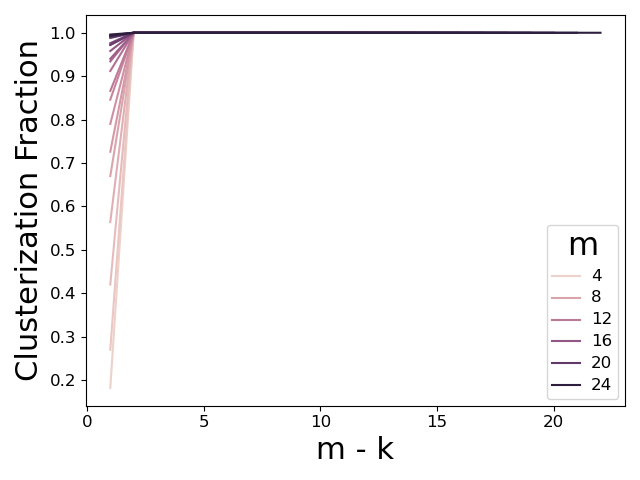
\includegraphics[height=0.5\textwidth]{../latex/figs/simulations.png}
    \caption{Fraction of clustered $A$ for $AA^t = M$ and $M$
      generated randomly (see text and repository for details on
      generating $M$). It is evident that when $m-k > 1$ clusterization
      is prevalent, whereas for lower $m-k$ clusterization is not.}
  \label{fig:sim_AAt}
\end{figure}

\subsection{Further comments}
\RC I have a number of further comments in regards to the results and the
overall presentation of the manuscript.


\RC D-optimal design vs. statistical recovery rates: being more
familiar with the statistical inverse problem literature than with
D-optimal design, the clusterisation phenomenon demonstrated in this
paper raises the question as to whether consistent recovery of the
unknown ($\param$ in the notation of this paper) is possible under
this choice. All the results I am aware of either assume white
noise/equally spaced design (e.g.~\cite{knapik2011}) or measurement
locations sampled uniformly at random (e.g.~\cite{nickl2023}). There
are also some results with more general design under conditions on the
fill-distance of the grid (e.g.~\cite{teckentrup2020}). All of these
specifically prevent clusterisation, which is key to the statistical
analysis. Hence, it is not clear to me even if D-optimal design should
be pursued at all, if it indeed it leads to clusterisation as implied
by the present paper. I think a discussion on this would be
illuminating for the reader and help draw a connection to the broader
statistical inverse problems literature.

\AR I added a discussion on this subject. In the manuscript this
discussion is broken in two since the second part relies on Theorem
\ref{thm:char}. Thus, the first part is in the Introduction and the
second part follows the statement and proof of the abovementioned
theorem.
\begin{quote}%%Convergence
  Clusterization in D-optimal designs raises the question of whether
  D-optimal designs should be pursued at all. While other authors have
  established convergence results for decaying measurement error
  \cite{knapik2011}, space-filling measurements \cite{teckentrup2020}
  and randomly sampled designs \cite{nickl2023}, their results do not
  hold for D-optimal designs. Luckily, we can expect convergence from
  D-optimal designs (including clustered designs) in the following
  sense: the posterior uncertainty ellipsoid will contract to zero
  along each one of its eigenvectors. See Section
  \ref{subsub:convergence} for a precise statement and a proof based
  on Theorem \ref{thm:char} --- the main theorem of this manuscript.
\end{quote}
\begin{quote}
  In this section we fulfill our promise from Section
  \ref{subsub:implications} and prove that the posterior uncertainty
  ellipsoid in $\hilo$ will contract to zero along every eigenvector
  of $\fwd \prcov \fwd^*$. In our proof we ignore potential problems
  with conducting inference on function spaces which are not unique to
  D-optimal designs (see e.g.~\cite{owhadi2015} for more details).
  \newline
  \newline  
  First, denote $\opt_m$ a D-optimal design utilizing $m$ measurements
  and denote $k_m := \rank\opt_m^*\opt_m$. An immediate consequence of
  Theorem \ref{thm:char} is that allowing more measurements will
  eventually allow us to measure each eigenvalue, i.e.:
  \begin{equation}\label{eq:lim}
    \lim_{m\to\infty} k_m = \infty
  \end{equation}
  \newline
  \newline
  Now, recall that part (5) of Theorem \ref{thm:char} ensures that the
eigenvalues of the posterior pushforward covariance equal
\begin{equation*}
  \theta^{(k)}_i = \left ( \frac{\sum_{j=1}^{k} \lambda_j^{-1} +
    \sigma^{-2}m}{k} \right )^{-1}, \text{ for $i\leq k$}.
\end{equation*}
Using the inequality for the arithmetic and harmonic means, it is easy
to verify that
\begin{equation*}
  \theta^{(k)}_i \leq \lambda_{k}.
   %% \leq \frac{\sum_{j=1}^{k} \lambda_j}{k}
\end{equation*}
Since $\lim_{k\to \infty} \lambda_k= 0$, we conclude that for all $i$,
$\lim_{k\to\infty} \theta^{(k)}_i = 0$. Combining the latter
observation with eq.~\eqref{eq:lim}, we conclude that
$\lim_{m\to\infty} \theta^{(k_m)}_i = 0$ for all $i$. Therefore,
posterior uncertainty decays to zero for all eigenvectors.
\end{quote}




\RC Figure 1: It is hard to discern whether the measurements locations
are perfectly overlapping or just very closely placed. Perhaps using
dots with numbers here would help the readability.
  
\AR It is impossible to visually discern the measurements, even when
resolution is increased. These measurements are not identical
numerically, but they are identical to five decimal digits. Since I
find these points via optimization over point location in
$\Omega=[0,1]$ I view a numerical error $<10^{-5}$ as reasonable.

\RC Experiment with the 1D heat equation: the experiment showcases
some interesting phenomena, but also raises many questions. For
instance: I would expect the dimensionality of the working domain
(here the unit interval $[0, 1]$) to play a role, since larger
dimension allow for higher freedom in placing the design points.
Further, a dimensionality effect should also arise directly from
Theorem 1\footnote{Now denoted Theorem \ref{thm:char}.} via the prior
covariance eigenvalues: in the experiment the prior covariance
operator is set to be equal to the inverse Laplace operator
$(-\Delta)^{-1}$. In d-dimensional domains, its eigenvalues
$\lambda_j$ are known to follow Weyl’s asymptotics, growing as
$j^{2/d}$, which should then impact the index after which the
eigenvalues are ‘thresholded’ by the procedure.

\AR These are two great points. Indeed, the growth of eigenvalues of
the Laplacian is different in higher dimensions. This is why in higher
dimensions we would have to take as prior \(u_0 \sim
\mathcal{N}(\param_0, (-\Delta)^{-\gamma})\), for some \(\gamma >
d/2\) in order to maintain regularity of prior realizations. I decided
not to include a discussion on the choice of priors in higher spatial
dimensions because (1) it would require too much exposition and make
me digress from the main points I wanted to convey and (2) due to
technical difficulties in installing packages for inverse problems
\cite{attia2023pyoed, villa2021} I had to implement the inverse
problem of the 1D heat equation from scratch, so I decided to leave
out experiments in higher dimensions.

  
\RC Also, it should be relatively easy here to also study empirically
the effect of the correlated error model in preventing
clusterisation. Investigating all these issues in the context of the
presented numerical set up would considerably enlarge the breath of
the present work.

\AR I added relevant simulations to a new section Numerical
Experiments:


\begin{quote}
  In order to verify the results of Section
  \ref{section:non_vanishing}, we run simulations of the inverse
  problem of the 1D heat equation with nonvanishing model error
  \(\modcov = \prcov^2 \). Indeed, including model correlation pushes
  measurements apart, see Fig.~\ref{fig:corr_errors}. Code generating
  Fig.~\ref{fig:corr_errors} is located in module
  \texttt{clusterization.py} in the accompanying
  \href{https://github.com/yairdaon/OED}{repository}.
\end{quote}
\begin{figure}
  \centering
  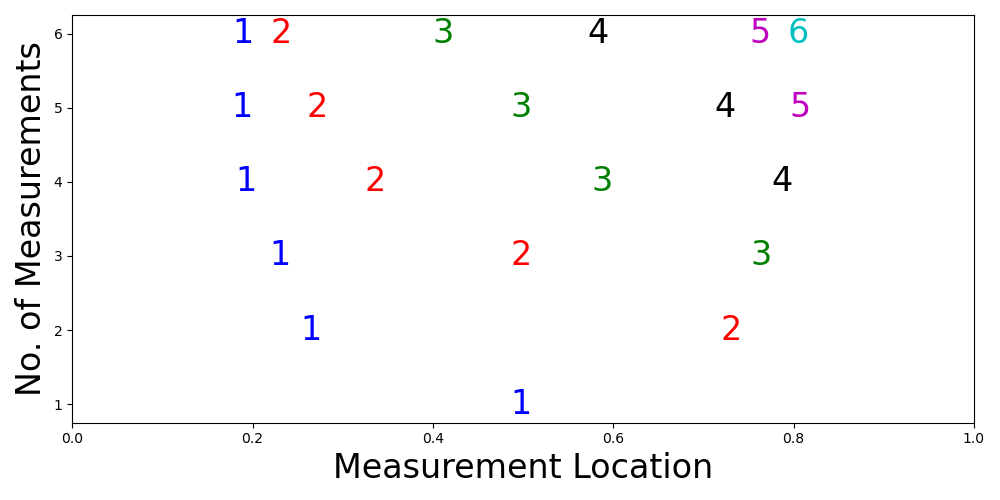
\includegraphics[height=0.5\textwidth]{../latex/figs/dst_modelError4.png}
  \caption{Model correlation mitigates clusterization. We add a
    model correlation term to the error terms in the 1D heat
    equation inverse problem. Lo and behold, measurements are not
    close anymore and are pushed away thanks to the model error
    term.}
    \label{fig:corr_errors}
\end{figure}

  
\RC I found very hard to understand Theorem 1 immediately at the end
of Section 1, as all the necessary background is introduced only
later. Since the same result is also stated and proved in Section 5, I
would consider cutting it from Section 1. The paragraphs in p.4 and 5
already do a good job presenting the results, and the repetition of
the formal statement does not seem necessary here.

\AR I removed the statement of Theorem 1 from the Introduction. It is
Theorem \ref{thm:char} now.


\RC Denoting the optimal design in Theorem 1 by simply $\obs$ is
somewhat confusing, cf.~the equation in the second item. Perhaps a
separate notation such as $\bar{\obs}$ would help readability.

\AR Thank you for the comment, I completely agree. Optimal designs are
now denoted $\opt$.

  
\RC Section 1.2 seems altogether unnecessary; the inverse regression
model considered in the paper are a modelisation of many real-world
phenomena, and they are routinely studied in statistical papers.

\AR I am glad you view this part as unnecessary, but I feel the model
might feel too abstract to some practitioners. Thus, I choose to keep
this part to avoid complaints from other readers.

\RC What does ‘strongly smoothing’ operator means in the third line of Section 2.1?

\AR Basically I meant that its eigenvalues decay "quickly". I
understand this is not a common or well-defined term so I removed the
relevant sentence.

  
\RC Section 4: the conclusion reached at the end of the section on
p.15 seem to imply that in the noiseless limit, repeating any
measurement does not improve the objective criterion, if correlated
error model are present.

\AR Indeed, this is very intuitive: when no observation error is
present, a repeated measurement does not tell us anything new.


\RC Is it clear however that adding any (non-repeated) measurement
always strictly increases it? I.e., there could be situations where
adding one measurement does not change the value of the optimised
criterion?

\AR Thanks for this insightful comment! Such cases are possible but I
view them as pathological. I added a short discussion reproduced
below:

\begin{quote}%% Pathologies
It is worth noting that by the nonnegativity of the KL divergence,
$\tar$ cannot decrease upon adding measurements. However, we can
construct examples where the posterior does not change upon taking a
new measurement e.g.~if the prior variance vanishes on some
eigenvector and a measurement is taken on said eigenvector. We do not
expect a measurement to generate no information gain whatsoever in any
realistic scenario, and ignore such pathologies.
\end{quote}

\RC Also, can the conclusion drawn here be extended to the case of
noisy observations $\sigma > 0$?

\AR I do not expect this conclusion to hold: if noise is present, even
a repeated measurement will result in some information gain and an
increase in design criterion. The reason is that for that particular
measurement the signal-to-noise ratio increases: observation error is
effectively reduced by a factor of $1/\sqrt{2}$ for the repeated
measurement. I discuss this briefly in the revised manuscript:
 
\begin{quote} %% Replication
  Clusterization should not be confused with replication. Replication
requires that the experimentalist executes multiple trials under
circumstances that are \emph{nominally identical} \cite[Section
  1.2.4]{morris2011}. Replication is commonly viewed as a beneficial
and even necessary aspect of optimal experimental design
\cite{fisher1949design, morris2011, schafer2001replication}.
For example, \cite{fisher1949design}, suggested repeating his famous
milk and tea experiment in order "to be able to demonstrate the
predominance of correct classifications in spite of occasional
errors". Unfortunately, in the experiments we consider, replication is
impossible. For example, in the MRI problem, we cannot generate an
individual nominally identical to the one we wish to scan.
\newline
\newline
Similarly to a design implementing replication, a clustered design
reduces the signal-to-noise ratio of the repeated measurements
\cite{telford2007brief}. The difference is that a clustered design
takes repeated measurements at the expense of other quantities not
measured at all. For example, consider an experiment measuring the
effect of rainfall on grass growth \cite{fay2000rainfall}. The
experiment involved four rainfall manipulation "treatments"
(i.e.~simulating different timing and quantity of rainfall), each
replicated three times over different plots of land. Indeed, it seems
reasonable for researchers to replicate the phenomenon they are trying
to study. A clustered design in such an experiment would imply the
researchers should take a repeated measurement \emph{on the same
plot}, at the expense of measuring grass growth in other plots!
\newline
\newline
To conclude our short discussion on replication vs.~clusterization:
these are fundamentally different concepts and even though replication
is quite intuitive, it is inapplicable to the inverse problems we
consider in this manuscript.
\end{quote}
  
  
\RC At the end of Section 4 on p.15 it is mentioned that $\tar$ is not
defined for $\sigma^2= 0$, but in the latter case, could not a
Gaussian posterior measure be still defined as in Gaussian process
regression, e.g~\cite{rasmussen2006}].

\AR Indeed, one can define a posterior, so a KL divergence from said
posterior to prior could be calculated and $\tar$ evaluated. However,
taking $\sigma = 0$ in Theorem 1 (the theorem of
\cite{AlexanderianGloorGhattas14}) gives $\tar \equiv \infty$. I did
not study this subject further.

  
\RC Theorem 1 is expressed in terms of the prior covariance matrix,
which is a user specified quantity. Hence, it seems to me that all
sort of design behavior under the D-optimal criterion can occur by
engineering the prior. It would perhaps be informative to study in
more details some representative example of inverse problem and
Gaussian prior. For example, the recovery of the initial condition
with the ‘Mat\'ern-like’ Gaussian prior laid out in the supplement are
good candidates.

\AR the Mat\'ern-like prior actually arises by using a Laplacian-like
operator as a prior \cite{rue2011}. So a study of this example (with
and without correlated errors) is already included in the paper. I am
afraid implementing another inverse problem is out of scope for the
present paper since I was not able to install common packages for
inverse problems \cite{attia2023pyoed, villa2021} on my machine.
  
\RC For these it is still not clear how the conclusion from Theorem 1
translates into the Figure 1, also because I am unsure about the
applicability of the result to point evaluations.

\AR Indeed, point evaluations $\delta_x$ are not in any function space
I consider in the paper since my analysis is limited to Hilbert
spaces. Point evaluations can be approximated well in
e.g.~$L^2(\Omega)$ so in my opinion this is not a deal breaker. For
example, we can replace point evaluations by $R(x;t) =
t\mathbf{1}_{[-1/2t, 1/2t]}(x)$, where $\mathbf{1}_{[a,b]}$ is an
indicator function on the interval $[a,b]$. We will then need to
change the norm constraints on measurement vectors from unit to
$\|R(\cdot;t)\|^2 = \int R^2(x;t)dx = t$ norm but that does not change
the analysis as long as $t$ is fixed. I barely mentioned this issue in
the paper since I think it is confusing and adds little context. See a
footnote I added:

\begin{quote} %% Footnote
  The alert reader will likely ask how do we reconcile point
  measurements $\delta_x$ as suggested by the formulation of the 1D
  heat equation with working in Hilbert spaces. We don't. We follow
  standard practice in the literature and restrict our analysis to
  Hilbert spaces. We can satisfy ourselves with the fact that point
  evaluations could be approximated in a standard Hilbert space like
  $L^2(\Omega)$.
\end{quote}
  
\RC In particular, how the conclusion that with $m = 4$ measurements
the D-optimal procedure will aim to ignore the third and fourth
eigenvalue/function was drawn?

\AR I added more details to the explaination explain in the revised
manuscript, see Section \ref{subsub:clusterization1}. See text
reproduced below.
\begin{quote}
Consider $\fwd$ and $\prcov$ from \emph{the inverse problem of the
heat equation}. As before, we denote the eigenvalues of
$\fwd\prcov\fwd^*$ by $\lambda_j$. We input these eigenvalues into our
\emph{generic} model, and find a D-optimal design $\opt$ for our
generic model using Theorem \ref{thm:char}. In our generic model, the
measurements we take are best utilized in reducing uncertainty for the
first $k$ eigenvectors. So, a D-optimal design arising from our
\emph{generic model} completely avoids measuring eigenvectors $k+1$
and above.
\newline \newline
Of course, in a real life problem --- such as the inverse problem of
the 1D heat equation --- it is likely impossible to find measurements
for which all eigenvectors $k+1$ and above are zero. However, if the
eigenvalues of $\fwd\prcov\fwd^*$ decay quickly (recall the
square-exponential decay for eigenvalues of the 1D heat equation in
eq.\eqref{eq:decay}), a D-optimal design will try to balance measuring
a small number (i.e.~$k$) of the leading eigenvectors.
%%\end{quote}
%%\begin{quote}
\newline \newline
The abovementioned balance is explored in
Fig.~\ref{fig:eigenvectors}. We allow $m=4$ measurements in $\Omega =
[0,1]$ and observe that D-optimal measurement locations are clustered
at $x_1 = 0.31$ and $x_2 = 0.69$. Upon close inspection of the scaled
eigenvectors of $\fwd \prcov \fwd^*$, we first observe that
eigenvectors $3$ and above have negligible prior amplitude. Since we
only have $m=4$ measurements at our disposal, we interpret these
results, following Theorem \ref{thm:char}, as implying we should only
care about measuring the first and second eigenvectors. Then, we note
the D-optimal $x_1,x_2$ present a compromise between the amplitude of
the first and second eigenvectors. For example, a measurement at
$x=0.5$ would have ignored the second eigenvector altogether, since
the second eigenvector is zero at $x=0.5$.
\newline \newline
Now we can understand measurement clusterization for the inverse
problem of the 1D heat equation. A D-optimal design attempts to
measure the first $k$ eigenvectors of $\fwd \prcov \fwd^*$. But there
may be (spatial) limitations on where these $k$ eigenvectors have
large amplitude. For the inverse problem of the heat equation there
are two spatial locations that present a good compromise between the
amplitudes of the first and second eigenvectors, namely $x_1$ and
$x_2$ --- see Fig.~\ref{fig:eigenvectors}. We have $m=4$ measurements
at our disposal but only two spatial locations that are a good
compromise between the amplitudes of the first and second scaled
eigenvectors. Thus, clusterization arises as a consequence of the
pigeonhole principle.
\end{quote}
\begin{figure}\label{fig:eigenvectors}
    \centering
    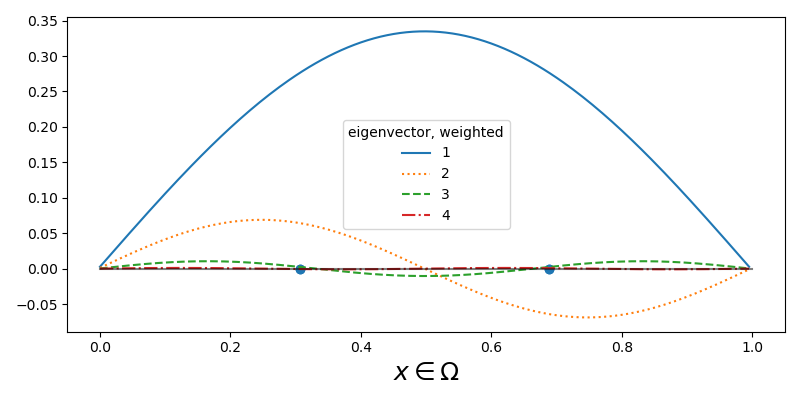
\includegraphics[width=\textwidth]{../latex/figs/eigenvectors_dst_scaled.png}
    \caption{D-optimal measurement locations ($m=4$ measurements) and
      weighted eigenvectors for finding the initial condition of the
      1D heat equation. Measurement locations and weighted
      eigenvectors are plotted over the computational domain $\Omega =
      [0, 1]$ (x-axis). Measurement clusterization occurs
      approximately at $0.31$ and $0.69$. These two locations are a
      compromise between the amplitudes of the first and second
      eigenvectors, which are the eigenvectors that a D-optimal design
      aims to measure. Allocating $m=4$ measurements into two
      locations results in clusterization, according to the pigeonhole
      principle.}
  \label{fig:why}
\end{figure}



%% \begin{quote}
%%   Building on Theorem \ref{thm:char}, we can now give a compelling
%%   explanation to the measurement clusterization we observed for the
%%   inverse problem of the heat equation, see Section
%%   \ref{subsub:clusterization1} below. We also suggest a generic
%%   explanation for clusterization, see Section
%%   \ref{subsub:clusterization2}.
%%   \newline
%%   \newline
%%   Consider $\fwd$ and $\prcov$ from \emph{the inverse problem of the
%%   heat equation}. As before, we denote the eigenvalues of
%%   $\fwd\prcov\fwd^*$ by $\lambda_j$. We input these eigenvalues into
%%   our \emph{generic} model, and find a D-optimal design $\opt$ for our
%%   generic model using Theorem \ref{thm:char}. In our generic model,
%%   the measurements we take are best utilized in reducing uncertainty
%%   for the first $k$ eigenvectors. So, a D-optimal design arising from
%%   our \emph{generic model} completely avoids measuring eigenvectors
%%   $k+1$ and above.
%%   \newline
%%   \newline
%%   Of course, in a real life problem --- such as the inverse problem of
%%   the 1D heat equation --- it is likely impossible to find measurement
%%   locations for which all eigenvectors $k+1$ and above are
%%   zero. However, if the eigenvalues of $\fwd\prcov\fwd^*$ decay
%%   quickly (recall the square-exponential decay for eigenvalues of the
%%   1D heat equation in eq.\eqref{eq:decay}), a D-optimal design will
%%   try to balance measuring a small number (i.e.~$k$) of the leading
%%   eigenvectors.
%% \end{quote}
%% \begin{quote}
%%   The abovementioned balance is explored in
%%   Fig.~\ref{fig:eigenvectors}. We allow $m=4$ measurements in $\Omega
%%   = [0,1]$ and observe that D-optimal measurement locations are
%%   clustered at $x_1 = 0.31$ and $x_2 = 0.69$. Upon close inspection of
%%   the scaled eigenvectors of $\fwd \prcov \fwd^*$, we first observe
%%   that eigenvectors $3$ and above have negligible prior
%%   amplitude. Since we only have $m=4$ measurements at our disposal, we
%%   interpret these results, following Theorem \ref{thm:char}, as
%%   implying we should only care about measuring the first and second
%%   eigenvectors. Then, we note the D-optimal $x_1,x_2$ present a
%%   compromise between the amplitude of the first and second
%%   eigenvectors. For example, a measurement at $x=0.5$ would have
%%   ignored the second eigenvector altogether, since the second
%%   eigenvector is zero at $x=0.5$.
%%   \newline
%%   \newline
%%   Now we can understand measurement clusterization for the inverse
%%   problem of the heat equation. A D-optimal design attempts to measure
%%   the first $k$ eigenvectors of $\fwd \prcov \fwd^*$. But there may be
%%   (spatial) limitations on where these $k$ eigenvectors have large
%%   amplitude. For the inverse problem of the heat equation there are
%%   two spatial locations that present a good compromise between the
%%   amplitudes of the first and second eigenvectors, namely $x_1$ and
%%   $x_2$ --- see Fig.~\ref{fig:eigenvectors}. We have $m=4$
%%   measurements at our disposal but only two spatial locations that are
%%   a good compromise between the first and second scaled
%%   eigenvectors. Thus, clusterization arises as a consequence of the
%%   pigeonhole principle.
%% \end{quote}

%% \begin{figure}\label{fig:eigenvectors}
%%   \centering
%%   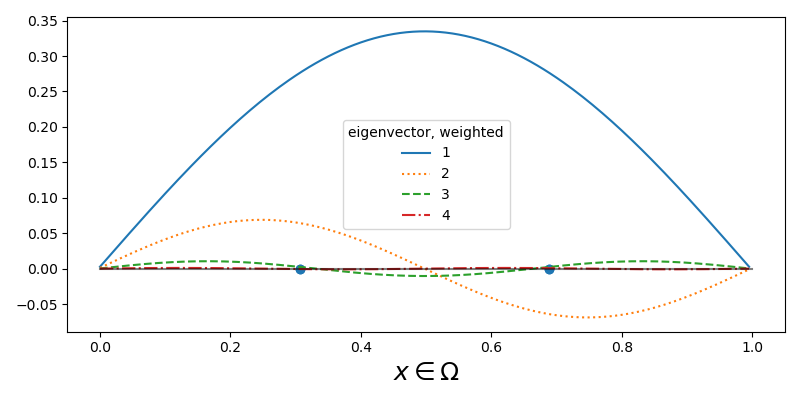
\includegraphics[width=\textwidth]{../latex/figs/eigenvectors_dst_scaled.png}
%%   \caption{D-optimal measurement locations ($m=4$ measurements) and
%%     weighted eigenvectors for finding the initial condition of the 1D
%%     heat equation. Measurement locations and weighted eigenvectors are
%%     plotted over the computational domain $\Omega = [0, 1]$
%%     (x-axis). Measurement clusterization occurs approximately at
%%     $0.31$ and $0.69$. These two locations are a compromise between
%%     the magnitudes of the first and second eigenvectors, which are the
%%     eigenvectors that a D-optimal design aims to measure. Allocating
%%     $m=4$ measurements into two locations results in clusterization,
%%     according to the pigeonhole principle.}
%%   \label{fig:why}
%% \end{figure}
 



\bibliographystyle{apalike}
\bibliography{../../lib.bib}

\end{document}
